
\section{Overview}\label{overview}


Im Lernteil des Mumie-Projektes unterteilt sich das
\textbf{Haupt}browserfenster in folgende Bereiche:

\begin{list_sabina}
        \item \textbf{zentrale Men"uleiste} (f"ur globale Optionen)
        \item \textbf{Navigationsbereich} (f"ur die interaktive Pr"asentation des speziellen Moduls)
        \item \textbf{zentrales Inhaltsfenster} (f"ur den inhaltlichen ``Hauptinput'')
\end{list_sabina}

\begin{figure}[h]
\begin{center}
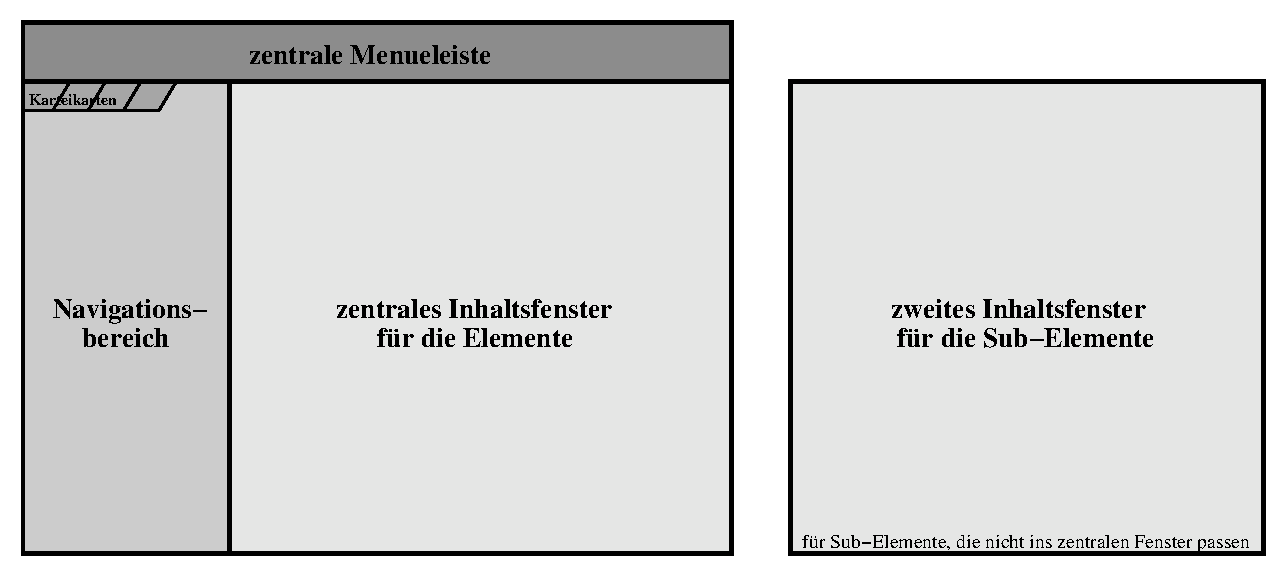
\epsfig{file=Skizzen/gesamtszenario_01.eps, height = 5cm} 
\caption{Layout der Hauptansicht im Lerntool}
\end{center}
\end{figure}


Der Navigationsbereich wird auf zwei verschiedene Weisen realisiert:

\begin{list_sabina}
        \item \textbf{Navigationsnetz}: Die Netzdarstellung erlaubt das orientierte
          Navigieren im gew"ahlten Kurs, stellt aber zus"atzlich weitere
          Elemente und alternative Wege dar, die jederzeit mit angew"ahlt
          werden k"onnen. \\
          Die Netzstruktur dient insbesondere der Vermittlung von
          mathematischen Zusammenh"angen: die logischen Abh"angigkeiten der
          Elemente werden durch eine Strichart (``logischer Pfad''), 
          der gew"ahlte Kurs durch eine zweite Strichart (``Kurspfad'')
          dargestellt. Forward/Backward-Aktionen beziehen sich stets
          auf den Kurspfad.
        \item \textbf{lineare Navigation:} Die lineare Darstellung (Modell
          etwa wie ein U-Bahn-Plan f"ur eine einzige Linie) stellt nur die
          Elemente des Modules dar, die f"ur den gew"ahlten Kurs vorgesehen
          sind. Alternative Wege und/oder weitere vorhandene Elemente sind in
          dieser Darstellung unsichtbar.\\
	  Die lineare Navigation dient insbesondere dem Ziel, dem 
	  ``Lost-in-Cyberspace''-Effekt entgegenzuwirken.
\end{list_sabina}


Ausgangspunkt f"ur die Darstellung ist zun"achst das Navigationsnetz (hier
wird auf Alternativen erst aufmerksam gemacht, deren Existenz anderenfalls
nicht sichtbar ist). Zwischen den beiden Navigationsformen kann zu jeden
Zeitpunkt geswitched werden (Karteikartensytem am oberen Rand des
Navigationsbereiches).


Im folgenden werden beide Navigationsbereiche im Detail beschrieben.

